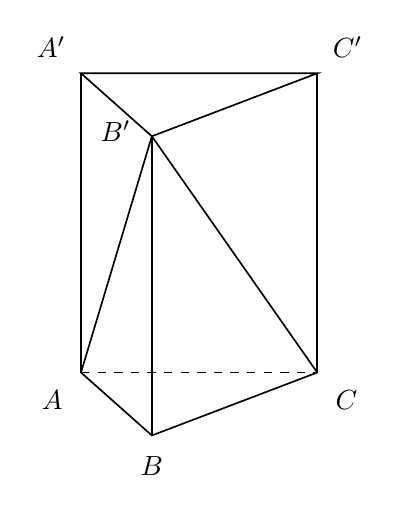
\begin{tikzpicture}[x=1cm,y=1cm,line width=.6pt,font=\normalsize]
\coordinate (A) at (0,0.4);
\coordinate (B) at (0.9,-0.4);
\coordinate (C) at (3.0,0.4);
\coordinate (Ap) at (0,4.2);
\coordinate (Bp) at (0.9,3.4);
\coordinate (Cp) at (3.0,4.2);
% prism frame
\draw (A) -- (Ap);
\draw (B) -- (Bp);
\draw (C) -- (Cp);
\draw (Ap) -- (Bp) -- (Cp) -- cycle;
\draw (A) -- (B) -- (C);
\draw[dashed] (A) -- (C);
% inner tetrahedron B'-A-C
\draw (Bp) -- (A);
\draw (Bp) -- (C);
\node[above left,xshift=-2pt,yshift=2pt] at (Ap) {$A'$};
\node[left,xshift=-4pt,yshift=2pt] at (Bp) {$B'$};
\node[above right,xshift=2pt,yshift=2pt] at (Cp) {$C'$};
\node[below left,xshift=-3pt,yshift=-3pt] at (A) {$A$};
\node[below,xshift=0pt,yshift=-4pt] at (B) {$B$};
\node[below right,xshift=3pt,yshift=-3pt] at (C) {$C$};
\end{tikzpicture}
